\section{Data Acquisition}
\label{sec:dataset}

\subsection{Acquisition and composition}
\label{sec:acquisition}

The \textsc{CrackID} dataset~\cite{ferramenta2026crackid} consists of 140 photographs of 17 exterior walls taken at a single site over four half-days using two consumer handheld devices (Fig.~\ref{fig:dataset-examples}).
The walls are either stippled render (textured) or smooth painted plaster, and the only visible defects are cracks.
Six walls are used for validation (01--06; 66 photographs, 66 identities) and eleven for testing (07--17; 74 photographs, 146 identities).
Only identities in at least two photographs are \emph{matchable} (18 validation, 19 test); their queries are the known (answerable) ones.
The \emph{frozen snapshot}, used for all results, comprises walls 01--17 of Version 1 of the released dataset~\cite{ferramenta2026crackid}. The \emph{live dataset} is the full current release, which also contains walls 18 and 19, added after the snapshot was frozen and excluded from results.
Each wall was photographed in a continuous walk-around (median 3~s between frames, max 81~s), so the data include within-visit viewpoint and scale changes.
This is more favorable than multi-visit matching, though not a formal upper bound.
The frozen snapshot has 439 known and 74 unknown validation queries, and 280 known and 258 unknown test queries. Positive query--gallery pairs number 26,012 (validation) and 5,722 (test); valid pairs (both instances annotated) number 89,118 and 31,822.
Of 301 same-wall test image pairs, 255 contain valid query--gallery pairs and 97 register (32\% of the 301); 15,328 of the 31,822 valid test pairs (48\%) belong to registered image pairs; we call these query--gallery pairs \emph{registered pairs}.

\subsection{Annotation}
\label{sec:annotation}

The labeling pipeline propagates each click frame-to-frame with ORB homographies, then merges fragments into physical-crack identities; this differs from the ORB matcher benchmarked in Table~\ref{tab:main}.
Merging is the main source of label risk, since an incorrect merge can turn a hard negative pair into a falsely labeled positive.
In the frozen snapshot, 95 of the 212 identities (45\%) result from merges, including 70 of the 146 test identities (48\%), with median bridged gaps of 228~px (test) and 286~px (validation).
One annotator reviewed all clicks, including 1,023 unclaimed points (not assigned to any identity): 45 were not cracks, 62 were placed off the crack on the surrounding wall, and 916 were cracks missed by the mask (Section~\ref{sec:method}). Inter-annotator agreement was not assessed.
This review reduces but does not eliminate merge risk. The live dataset must not be combined with the frozen figures without re-running the benchmark.

\begin{figure}[t]
\centering
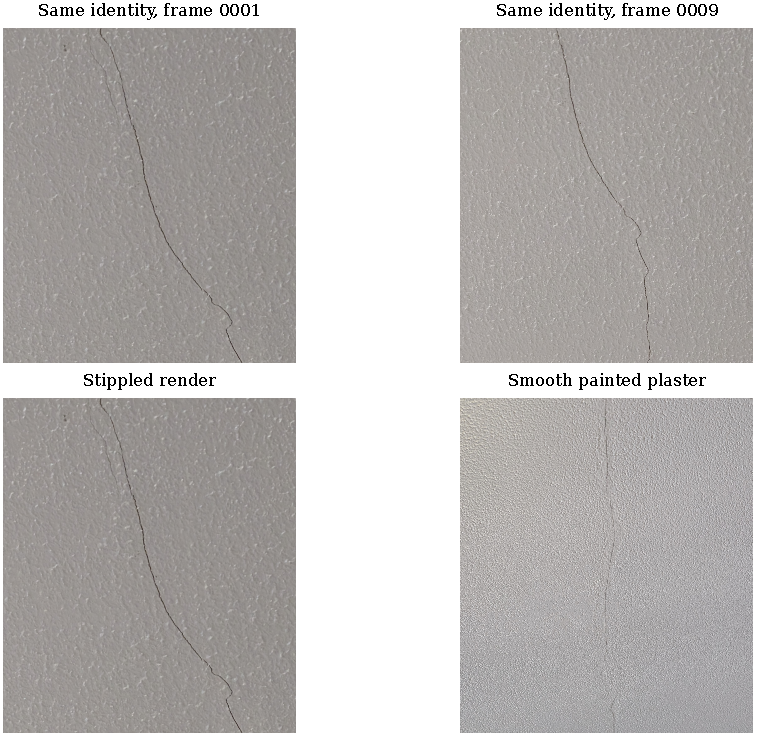
\includegraphics[width=0.5\columnwidth]{figs/dataset_examples.pdf}
\caption{\textsc{CrackID} examples. Top: one identity across non-adjacent frames. Bottom: stippled render versus smooth plaster. Labels were propagated via homographies and reviewed by a single annotator.}
\label{fig:dataset-examples}
\end{figure}
